%-------------------------------------------------------------------------------
\documentclass{article}

%-------------------------------------------------------------------------------
% Packages

% Translation
\usepackage[brazilian]{babel}

% General
\usepackage{amsmath}
\usepackage{environ}
\usepackage{graphicx}
\usepackage[margin=1in]{geometry}
\usepackage{minted}
\usepackage{xcolor}

% To-do List
\usepackage{amssymb}
\usepackage{pifont}
\usepackage{enumitem}

% Other
\usepackage{hyperref}
\usepackage[brazilian]{cleveref} % Must be after hyperref


% Custom lists
\newlist{todolist}{itemize}{2}
\setlist[todolist]{label=$\square$}
\newcommand{\done}{%
    \rlap{$\square$}{%
        \raisebox{2pt}{\large\hspace{1pt}\ding{51}
    }}\hspace{-2.5pt}
}

%-------------------------------------------------------------------------------
% User-commands
\newcommand{\todo}[1]{{\color{red}{#1}}}

\NewEnviron{superframe}{%
    \begin{center}
        \fbox{\setlength{\fboxsep}{1em}\fbox{\parbox{5.5in}{%
            \BODY{}
        }}}
    \end{center}
}

\NewEnviron{answer}{%
    \begin{samepage}
        \begin{solution}
            \BODY{}
        \end{solution}
    \end{samepage}
}

%-------------------------------------------------------------------------------
% Project configs
\title{%
    Segurança em Computação \\
    Trabalho Individual III
}
\author{João Paulo Taylor Ienczak Zanette}
\date{\today}

%-------------------------------------------------------------------------------
\begin{document}
    \maketitle{}

    %-------------------------------------------------------------------------
    \section{Parte 1}

    \begin{superframe}
        1. Criar certificado PGP\@.
        Obs: salvar a chave privada e não esquecer senha.


        Faça um backup da sua chave privada;
        Publicar a chave pública em um repositório GPG\@. Exemplos:
        \begin{itemize}
            \item Keyserver da RNP (use o Google para encontrar o site)
            \item MIT PGP Public Key Server
            \item Keyserver PGP.com
        \end{itemize}

        \textbf{Resultado Esperado:}

        \begin{todolist}
            \item[\done] Certificado do aluno publicado no repositório PGP\@.
        \end{todolist}
    \end{superframe}

    %-------------------------------------------------------------------------
    \section{Parte 2}

    \begin{superframe}
        2. Crie um novo certificado GPG para este trabalho individual (Não use
        o seu certificado pois este novo será revogado). Coloque esse
        certificado de testes no servidor GPG\@. Depois verifique seu status.
        Então, crie um certificado de revogação e revogue o certificado de
        testes.

        Resultado Esperado:

        \begin{todolist}
            \item[\done] Faça um relatório do que você fez, incluindo o KeyID
                do certificado revogado.
        \end{todolist}
    \end{superframe}

    Primeiramente, foi criada a chave GPG exatamente da mesma forma que foi
    feito para a Parte 1, ou seja, a partir da linha de comando foi executado:

    \begin{minted}[autogobble]{console}
        $ gpg --full-generate-key  # Geração da chave
        $ gpg --armor --export 5B1B5A3BD6CEE72D # Mostrar a chave pública no terminal
    \end{minted}

    Em seguida, no site do servidor de chaves da RNP foi adicionada, podendo
    ser buscada em \url{http://keyserver.cais.rnp.br:11371/} utilizando o ID
    (\texttt{0x5B1B5A3BD6CEE72D}). Em seguida, foi gerado um certificado de
    revogação, importado e enviado ao servidor de chaves da RNP:

    \begin{minted}[autogobble]{console}
        $ gpg -o revokee.asc --gen-revoke --armor 5B1B5A3BD6CEE72D
        $ gpg --import revokee.asc
        $ gpg --keyserver keyserver.cais.rnp.br --send-keys 5B1B5A3BD6CEE72D
    \end{minted}

    Depois de feitos todos esses passos, ao se tentar ver sobre as chaves
    guardadas localmente, é possível ver que a revogação foi satisfeita:

    \begin{minted}[autogobble,breaklines]{console}
        $ gpg --list-secret-keys --keyid-format LONG
        /home/jptiz/.gnupg/pubring.kbx
        ------------------------------
        sec   rsa2048/C598C13DF4964793 2019-04-26 [SC]
              48F1744C8CCB4C04A7A6F2B9C598C13DF4964793
        uid                 [ultimate] João Paulo Taylor Ienczak Zanette (For educational purposes) <jpaulotiz@gmail.com>
        ssb   rsa2048/B11690E2A8DDA995 2019-04-26 [E]

        sec   rsa2048/5B1B5A3BD6CEE72D 2019-04-26 [SC] [revoked: 2019-04-26]
              F6055CCED33CE15CC2A8065A5B1B5A3BD6CEE72D
        uid                 [ revoked] João Paulo Taylor Ienczak Zanette (More educational purpooooooses) <jpaulotiz@gmail.com>

        sec   rsa2048/1DFE185BDCAE898A 2019-04-29 [SC]
              BC50CCDA2D2DBAD0302EFEAD1DFE185BDCAE898A
        uid                 [ultimate] João Paulo Taylor Ienczak Zanette (Forgot last password :P For studying purposes.) <jpaulotiz@gmail.com>
        ssb   rsa2048/79D4F9460C7144E8 2019-04-29 [E]
    \end{minted}

    Também é possível ver a confirmação acessando
    \url{http://keyserver.cais.rnp.br:11371/} (\Cref{fig:revokee}).

    \begin{figure}[ht]
        \centering
        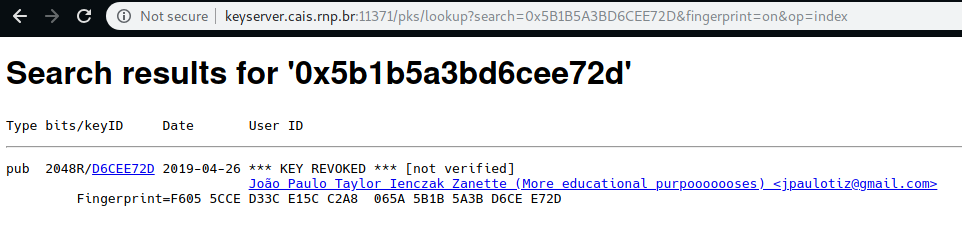
\includegraphics[keepaspectratio,width=1\textwidth]{revoked-keyserver.png}
        \caption{%
            Confirmação da revogação do certificado
            \texttt{5B1B5A3BD6CEE72D}.\label{fig:revokee}
        }
    \end{figure}

    %-------------------------------------------------------------------------
    \section{Parte 3}

    \begin{superframe}
        3. Pratique a revogação de assinaturas e certificados GPG\@. Assine um
        certificado qualquer GPG (de outra pessoa). E envie esse certificado
        para o servidor GPG\@. Depois verifique o status do certificado. E
        então, revogue a assinatura que você fez. Confira o resultado no
        servidor GPG\@.

        \begin{todolist}
            \item Faça um relatório do que você fez, incluindo o KeyID do
                certificado cuja assinatura você revogou.
        \end{todolist}
    \end{superframe}

    \begin{enumerate}
        \item Foi importada a chave de ``Adriano Tosetto'' pelo servidor do RNP
            (salva em um arquivo~.asc e então importada com \texttt{gpg
            --import <arquivo>.asc});
        \item Em seguida, foram executados os comandos para assinar e gerar um
            arquivo de assinatura:

            \begin{minted}[autogobble]{console}
                $ gpg --local-user 1DFE185BDCAE898A --sign-key adriano.rafael10@hotmail.com
                $ gpg --output ~/tosetto-signed.key --export --armor adriano.rafael10@hotmail.com
            \end{minted}

        \item O conteúdo do arquivo \texttt{tosetto-signed.key} foi enviado ao
            servidor da RNP como uma chave, confirmando a assinatura
            (\Cref{fig:revokee-sign});
        \item A assinatura foi revogada localmente utilizando:

            \begin{minted}[autogobble]{console}
                $ gpg --edit-key 52A4FF6D1F0CC9B8 # Editar a chave
                gpg> revsig
                Your decision? 0
                Enter an optional description; end it with an empty line:
                > My teacher asked. Sorry :(
                >
                Is this okay? (y/N) y
                gpg> Save changes? (y/N) y
                $ gpg --send-key 52A4FF6D1F0CC9B8 # Enviar chave ao servidor da RNP
                gpg: sending key 52A4FF6D1F0CC9B8 to hkps://hkps.pool.sks-keyservers.net
                $ gpg --recv-key 52A4FF6D1F0CC9B8 # Atualizar dados da chave
            \end{minted}
        \item Após isso, é acessando o site é possível ver que a assinatura foi
            revogado (\Cref{fig:revokeed-sign}).
    \end{enumerate}

    \begin{figure}[h]
        \centering
        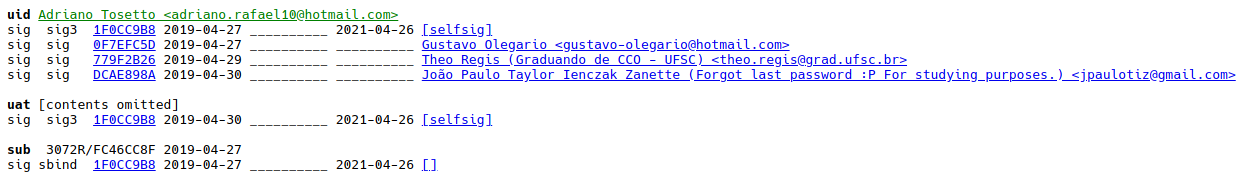
\includegraphics[keepaspectratio,width=1\textwidth]{tosetto-signed}
        \caption{%
            Certificado de Adriano Tosetto assinado.\label{fig:revokee-sign}
        }
    \end{figure}

    \begin{figure}[h]
        \centering
        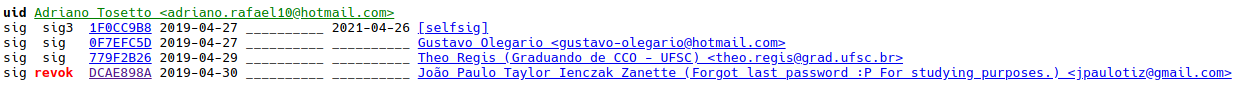
\includegraphics[keepaspectratio,width=1\textwidth]{tosetto-revoked-sig}
        \caption{%
            Certificado de Adriano Tosetto com assinatura
            revogada.\label{fig:revokeed-sign}
        }
    \end{figure}

    %-------------------------------------------------------------------------
    \section{Parte 4}

    \begin{superframe}
        4. O que é o anel de chaves privadas? Como este está estruturado? Na
        sua aplicação GPG onde este anel de chaves é armazenado? Quem pode ser
        acesso a esse porta chaves?
    \end{superframe}

    %-------------------------------------------------------------------------
    \section{Parte 5}

    \begin{superframe}
        5. Qual a diferença entre assinar uma chave local e assinar no
        servidor?
    \end{superframe}

    %-------------------------------------------------------------------------
    \section{Parte 6}

    \begin{superframe}
        6. O que é e como é organizado o banco de dados de confiabilidade?
    \end{superframe}

    %-------------------------------------------------------------------------
    \section{Parte 7}

    \begin{superframe}
        7. O que são e para que servem as sub-chaves?
    \end{superframe}

    %-------------------------------------------------------------------------
    \section{Parte 8}

    \begin{superframe}
        8. Coloque sua foto (ou uma figura qualquer) que represente você em seu
        certificado GPG\@.
    \end{superframe}

    %-------------------------------------------------------------------------
    \section{Parte 9}

    \begin{superframe}
        9. O que é preciso para criar e manter um servidor de chaves GPG,
        sincronizado com os demais servidores existentes?
    \end{superframe}

    %-------------------------------------------------------------------------
    \section{Parte 10}

    \begin{superframe}
        10. Dê um exemplo de como tornar sigiloso um arquivo usando o GPG\@.
        Envie esse arquivo para um colega e que enviar para você outro arquivo
        cifrado. Você deve decifrar e recuperar o conteúdo original.
    \end{superframe}

    %-------------------------------------------------------------------------
    \section{Parte 11}

    \begin{superframe}
        11. Mostre um exemplo de como assinar um arquivo (assinatura anexada e
        outro com assinatura separada), usando o GPG\@. Envie uma mensagem
        assinada para um colega. Esse colega deve enviar para você outra
        mensagem assinada. Verifique se a assinatura está correta.
    \end{superframe}
\end{document}
